\documentclass[a4paper,11pt]{article}
% --------------------------------------------------------------------------------------------------------> PACKAGES <--- %
\usepackage[frenchb]{babel}
\usepackage[utf8]{inputenc}
\usepackage{url}
\usepackage{graphicx}
\usepackage{tabularx}
\usepackage{eurosym}
%\usepackage{epsfig}
\usepackage{bibtopic}
\usepackage{comment}
\usepackage{tikz}
\usepackage{amsmath}

% --------------------------------------------------------------------------------------------------------> META DATAS <--- %
\usepackage[
  colorlinks=false,
  pdfborder={0 0 0},
  pdfauthor={Emmanuel Roubin},
  pdftitle={Roubin Emmanuel | Curriculum Vitae},
  pdfsubject={Curriculum Vitae},
  pdfkeywords={Materiaux a matrice cimentaire, Milieux heterogenes, Modele morphologique, Modelisation multi-echelles, Embedded Finite Element Method},
  pdfproducer={LaTeX with hyperref package},
  pdfcreator={latex, dvips, ps2pdf}
]{hyperref}

% --------------------------------------------------------------------------------------------------------> MARGIN <--- %
\pagestyle{empty}
\usepackage{vmargin}
\setmarginsrb{1.cm}{1.5cm}{1.5cm}{1.cm}{0cm}{0cm}{0cm}{0cm}

% --------------------------------------------------------------------------------------------------------> TITLE <--- %
\newcommand{\titre}[1]{
  \begin{center}
    \rule{0.4\textwidth}{0.5pt}
    \par\vspace{0.1cm}
    \textsc{\large #1}
    \par\vspace{-0.2cm}
    \par\noindent\rule{0.4\textwidth}{0.5pt}
  \end{center}
}

% --------------------------------------------------------------------------------------------------------> BEGIN DOCUMENTS <--- %
\begin{document}
\begin{center} \par\textsc{\huge Curriculum Vit\ae} \end{center}
\begin{minipage}{0.7\linewidth}
  \begin{flushleft}
    \LARGE Emmanuel ROUBIN \normalsize  \vspace{0.1cm} \\
    \large Docteur diplômé de l'École Normale Supérieure de Cachan\\
    \large Maître de conférence à l'Université Grenoble Alpes \normalsize\\\vspace{0.2cm}
    
    IUT 1, Département GCCD, Bureau 014\\
    151 rue de la Papeterie, 38 402 Saint-Martin-d'Hères\\
    \href{mailto:emmanuel.roubin@univ-grenoble-alpes.fr}{emmanuel.roubin@univ-grenoble-alpes.fr} $|$ 04 76 82 53 44 \\
    
    \vspace{0.2cm}  
    Laboratoire 3SR, Bâtiment Galilée, Bureau 228\\
    1270 rue de la Piscine, 38 400 Saint-Martin-d'Hères\\
     \href{mailto:emmanuel.roubin@3sr-grenoble.fr}{emmanuel.roubin@3sr-grenoble.fr} $|$ 04 56 52 86 49\\
    
  \end{flushleft}
\end{minipage}
\hfill
\begin{minipage}{4cm}
  %\centering \fbox{\href{http://perso.crans.org/roubin}{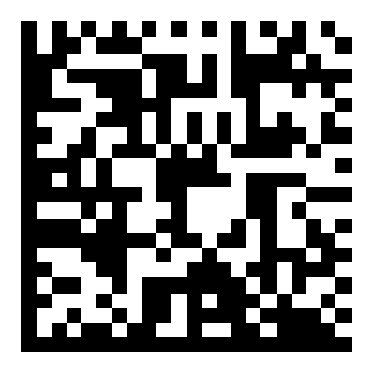
\includegraphics[width=3cm]{img/flashcode.eps}{}}}\\\vspace{0.1cm} \footnotesize\href{http://perso.crans.org/roubin}{perso.crans.org/roubin}
  \centering
  \fbox{\href{http://perso.crans.org/roubin}{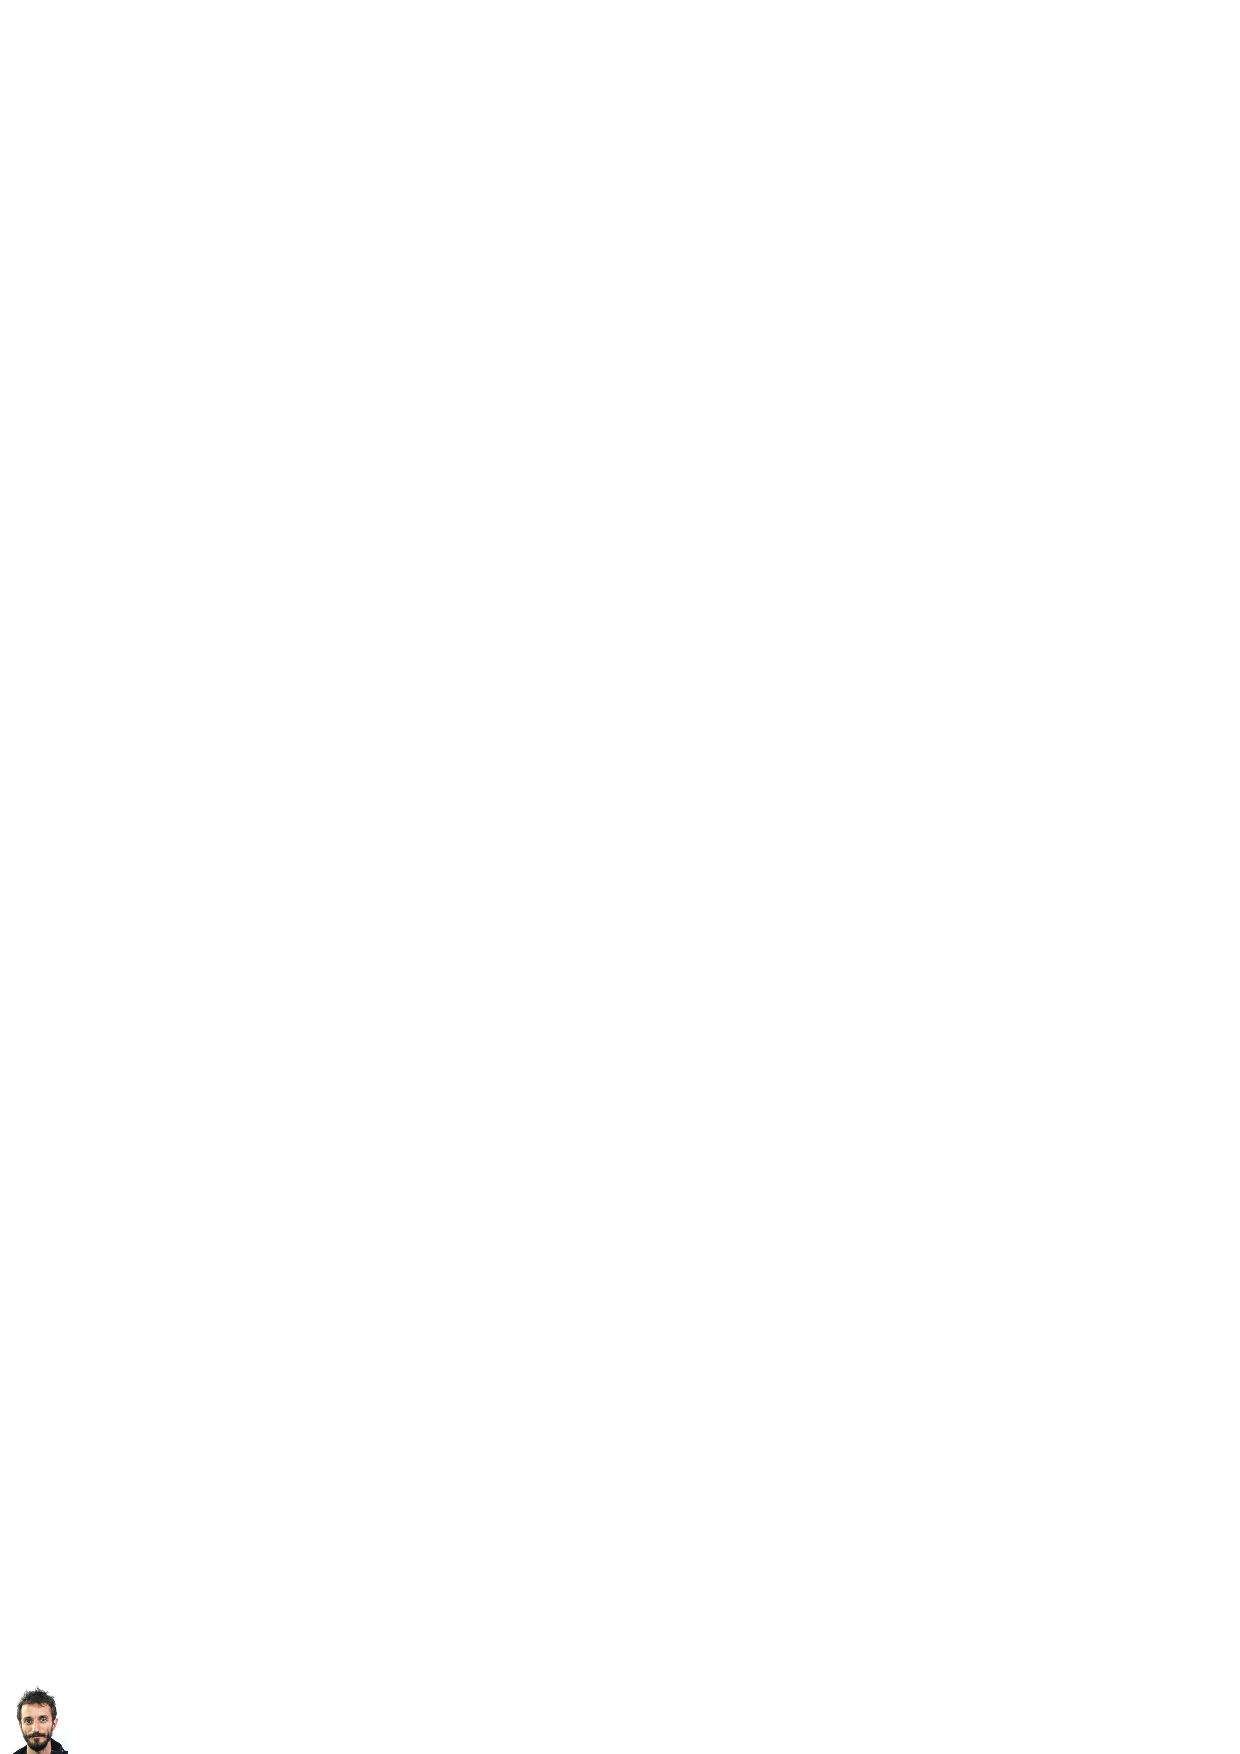
\includegraphics[width=3cm]{img/id.png}{}}} \\ \vspace{0.1cm}
  \footnotesize\href{http://perso.crans.org/roubin}{perso.crans.org/roubin}
\end{minipage}
\vspace{0.5cm}
%\begin{center}
%  \textsc{Profil : Chercheur en Génie Civil / Numéricien / Ancien moniteur de l'ENS Cachan}
%\end{center}

% --------------------------------------------------------------------------------------------------------> PARCOURS <--- %
\titre{Parcours}
\noindent\begin{tabular}{p{0.2\textwidth}p{0.75\textwidth}m{0.1\textwidth}}
  Depuis Sept. 2015 & \textbf{Maître de conférence} de l'Université Grenoble Alpes (UGA). Enseignant à l'IUT 1 GCCD rattaché au laboratoire 3SR.\hfill \raisebox{-0.2cm}{\includegraphics[height=0.6cm]{img/3sr.png}\includegraphics[height=0.6cm]{img/iut1_h.png}}\\
  Oct. 2013 à Juin 2015 & \textbf{Post-doctorant à l'International Center for Numerical Methods in Engineering (CIMNE)}, UPC Barcelone (Espagne), avec le Professeur X. Oliver. Travail au sein de l'équipe du projet ERC \emph{Advanced tools for computational design of engineering materials}  \hfill \raisebox{-0.2cm}{\includegraphics[height=0.6cm]{img/cimne.png}}\\
  Octobre 2013  & \textbf{Docteur} de l'ENS~Cachan. Sujet : \textit{Modélisation EF et morphologique de milieux hétérogènes à l'échelle mésoscopique : applications aux matériaux à matrice cimentaire}. Doctorat effectué sous la direction \href{http://lml.univ-lille1.fr/lml/?page=15&manID=1839}{J.-B. Colliat (LML, Lille)} au LMT-Cachan. Thèse soutenue à l'ENS Cachan le 10/10/2013 devant le jury composé de N. Burlion (président), D. Kondo (examinateur), J.-M. Torrenti (examinateur), X. Oliver, N. Benkemoun et J.-B. Colliat. \hfill \raisebox{-0.2cm}{\includegraphics[height=0.6cm]{img/lmt.jpg}} \\ 
  Mai - Juin 2012  &  \textbf{Séjour à l’Institut für Wissenschaftliches Rechnen}, TU Braunschweig (Allemagne), avec le Professeur H.G. Matthies. \hfill \raisebox{-0.2cm}{\includegraphics[height=0.6cm]{img/wire.jpg}} \\
  Sept. 2011 à 2013 & \textbf{Doctorant} chargé d'une \textbf{mission d'enseignement} à l'ENS~Cachan (128h)\\ 
  Sept. 2010 à 2011 & \textbf{Doctorant} et \textbf{vacataire} à l'ENS~Cachan (56h)\\ 
  Juin 2010      & \textbf{Diplôme de Master Recherche Génie Civil} de l'ENS~Cachan : Structures, Ouvrages et Matériaux dans leur environnement\\
                 & \textbf{Diplôme de l'ENS~Cachan}\\ 
  Mars - Juin 2010 & \textbf{Stage de recherche} (M2) au LMT-Cachan. Sujet : \textit{Modélisation morphologique des matériaux hétérogènes} sous la direction de J.-B. Colliat.\\
  Mai - Juillet 2009 & \textbf{Stage de recherche} (M1) à l'Université de Canterbury (Nouvelle-Zélande). Sujet : \textit{Evaluation of Screws Used in Laminated Veneer Lumber Rocking Connections} sous la direction de A.H. Buchanan. \hfill \raisebox{-0.2cm}{\includegraphics[height=0.6cm]{img/uc.jpg}} \\
  Septembre 2006 & Élève \textbf{professeur stagiaire} à l'ENS~Cachan (normalien)\par Physique appliquée puis Mécanique, Génie Civil. \hfill \raisebox{-0.2cm}{\includegraphics[height=0.6cm]{img/cachan.png}} \\
  De 2004 à 2006 &  \textbf{Classes préparatoires} PT/PTSI (Lycées Vauvenarges, Aix-en-Provence)
\end{tabular}
\vfill

% --------------------------------------------------------------------------------------------------------> ENSEIGNEMENT <--- %
\titre{Activités pédagogiques}
\begin{itemize}
\item[Depuis 2016] \textbf{Direction des \'Etudes} $1^\text{er}$ et $2^\text{ème}$ années IUT 1 GCCD  
\item[Depuis 2015] \textbf{MCF} à l'IUT 1 GCCD de l'Université Grenoble Alpes
  \begin{itemize}
  \item géotechniques, dimensionnement chaussées
  \item éclairage public, Projets de Fin d'Etude
  \end{itemize}
\item[2010 - 2013], \textbf{vacataire} puis chargé d'une \textbf{mission d'enseignement} à l'ENS Cachan et à l'UPMC (Jussieu Paris VI) pour un total de \textbf{184h eq. TD}. (Probabilité et incertitudes, Mécanique des Milieux Continus, Méthodes numériques, Mécanique probabiliste).
\end{itemize}
\vfill

\newpage
% --------------------------------------------------------------------------------------------------------> RECHERCHE <--- %
\titre{Activités de recherche}
% ---> MCF <---
\begin{itemize}
  \item[\textbf{Thématiques}] : Modélisation numérique du comportement des bétons
    \begin{itemize}
    \item Modélisation du caractère aléatoire de la \textbf{morphologie} (inclusions, porosité, percolation)
    \item Analyse \textbf{multi-échelles} et \textbf{multi-physiques}
    \item Modélisation de la \textbf{fissuration} et procédures de \textbf{réduction de modèles}
    \end{itemize}
  \item[\textbf{Projets}] :
  \item 2015 - : Participation à l'ANR MOSAIC \textit{``MesOscopic Scale durAbility Investigations for Concrete''} portée par J.-B Colliat.
  \item 2013 - 2015 : Participation au projet Européen ERC \textit{``Advanced tools for computational design of engineering materials''} porté par X. Oliver en tant que post-doctorant.
  \item[\textbf{Encadrements de thèses}] :
  \item Olga Stamati (Grenoble, 3SR, 2016-) : \textit{``Investigations expérimentales et numériques du comportement des matériaux à matrice cimentaires sous fort confinement : Lien avec l'imagerie 3D''}
  \item Yue Sun (Lille, LML, 2016-) : \textit{``Investigations expérimentales et numériques du comportement des matériaux à matrice cimentaires sous fort confinement : Lien avec l'imagerie 3D''}
  \item Paul Hauseux (Lille, LML, 2012-2015) : \textit{``Modélisation de la fissuration et propagation des incertitudes au travers de Méthodes Éléments Finis: Applications à des probèmes d'excavation.''}
  \item[\textbf{Encadrements de stage de Master}] : Mateusz Bogdan (Cachan, LMT, 2011), Hala Damerji (Grenoble, 3SR, 2016), Olga Stamati (Grenoble, 3SR, 2016)
  %\item Thèse Alexis Vallade (LML, 2012-2016) : \textit{``Modélisation multi-échelle du gaz de schiste. Influence de la microstructure sur les propriétés macroscopiques et le procesus de fracturation.''}
  %\item Stage M2 Olga Stamati (3SR, 2016) : \textit{From x-ray tomography to FE simulation of cementitious materials: Making the link with quantitative image analysis}
  %\item Stage M2 Hala Damerji (3SR, 2016) : \textit{Mesoscale modeling of concrete failure under dynamic loading: Application to spalling test}
  %\item Stage M2 Mateusz Bogdan (LMT, 2011) : \textit{Modèle morphologique d'hydratation de matrices cimentaires} 
  \item[\textbf{Principales contributions}] :
    \begin{btSect}[bibperso/chrono]{bibperso/Published_top_five}
      \btPrintAll
    \end{btSect}
  \item[\textbf{Principales conférences}] : WCCM (Espagne, 2014), WCCM (Brésil, 2012), COMPLAS (Espagne, 2011)
\end{itemize}
\vfill      

% --------------------------------------------------------------------------------------------------------> COMPETENCES <--- %
\titre{Compétences}
\begin{tabular}{p{0.18\textwidth}b{0.01\textwidth}p{0.8\textwidth}}
  \textbf{Langues} & : & \textbf{Fran\c cais} (natif), \textbf{Anglais} (courant) et Espagnol\\
  \textbf{Programmation} & : & $C$, $C++$, Fortran77, Python2.7, Bash, Web (PHP, MySql)\\
  \textbf{Logiciels} & : & Feap (code EF), ParaView (post-process), environnement Unix/Linux\\
  \textbf{Edition} & : & \LaTeX, Keynote, Web (html5, css3, Jquery)
\end{tabular}
\vfill

% --------------------------------------------------------------------------------------------------------> INVESTISSEMENTS <--- %
\titre{Activités diverses}

\begin{tabular}{lcp{0.8\linewidth}}
  2014      & : & Développement du site internet d'apprentissage du fran\c{c}ais \href{http://e2lf.fr}{E2LF}\\
  2010      & : & Développement du site internet de \href{http://www.ecoba.ens-cachan.fr/index.php?part=acces}{l'ANR blanc ECOBA}\\
  2008      & : & Assistant régisseur lunière à l'Européen (Paris)\\
  2007-2008 & : & Président de deux associations culturelles (BdA/SdA Cachan)\\ 
  2007      & : & Elaboration et réalisation d'un projet éducatif en Inde (Hoé-Inde)\\
\end{tabular}

\vspace{0.5cm}
\begin{tabular}{lcp{0.8\linewidth}}
  \textbf{Sport} & : & Escalade et sports de haute-montagne\\
  \textbf{Musique} & : & Médaille d'or du conservatoire  Darius Milhaud en violoncelle (Aix-en-Provence 2004)
%                   &  & saxophone
%  \textbf{Autre} & : & Speedcuber, Webmaster, Régie lumière, photographie
\end{tabular}

\vfill
\empty
	
\end{document}
